\documentclass{beamer}
\usetheme{Madrid}
\usepackage{tikz}
\title{Slides}\author{Me}\date{2026}
\begin{document}
\begin{frame}\titlepage\end{frame}
\begin{frame}{A frame}
\begin{itemize}\item<1-> One \item<2-> Two\end{itemize}
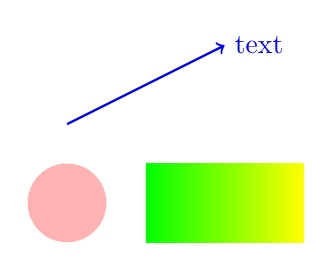
\begin{tikzpicture}
\draw[thick,->,blue] (0,0) -- (2,1) node[right]{text};
\fill[red!30] (0,-1) circle (0.5);
\shade[left color=green,right color=yellow] (1,-1.5) rectangle (3,-0.5);
\end{tikzpicture}
\end{frame}
\end{document}
